% --------------------------------------------------------------------------- %
% Poster for the ECCS 2011 Conference about Elementary Dynamic Networks.      %
% --------------------------------------------------------------------------- %
% Created with Brian Amberg's LaTeX Poster Template. Please refer for the     %
% attached README.md file for the details how to compile with `pdflatex`.     %
% --------------------------------------------------------------------------- %
% $LastChangedDate:: 2011-09-11 10:57:12 +0200 (V, 11 szept. 2011)          $ %
% $LastChangedRevision:: 128                                                $ %
% $LastChangedBy:: rlegendi                                                 $ %
% $Id:: poster.tex 128 2011-09-11 08:57:12Z rlegendi                        $ %
% --------------------------------------------------------------------------- %
\documentclass[a0paper,portrait]{baposter}

\usepackage{relsize}		% For \smaller
\usepackage{url}			% For \url
\usepackage{epstopdf}	% Included EPS files automatically converted to PDF to include with pdflatex

\usepackage{tikz}
\usetikzlibrary{shapes,arrows}

%%% Global Settings %%%%%%%%%%%%%%%%%%%%%%%%%%%%%%%%%%%%%%%%%%%%%%%%%%%%%%%%%%%

\graphicspath{{pix/}}	% Root directory of the pictures 
\tracingstats=2			% Enabled LaTeX logging with conditionals

%%% Color Definitions %%%%%%%%%%%%%%%%%%%%%%%%%%%%%%%%%%%%%%%%%%%%%%%%%%%%%%%%%

%\definecolor{bordercol}{RGB}{40,40,40}
%\definecolor{headercol1}{RGB}{186,215,230}
%\definecolor{headercol2}{RGB}{80,80,80}
%\definecolor{headerfontcol}{RGB}{0,0,0}
%\definecolor{boxcolor}{RGB}{186,215,230}

\definecolor{bordercol}{RGB}{186,215,230}
\definecolor{headercol1}{RGB}{186,215,230}
\definecolor{headercol2}{RGB}{186,215,230}
\definecolor{headerfontcol}{RGB}{40,40,40}
\definecolor{boxcolor}{RGB}{186,215,230}

%%%%%%%%%%%%%%%%%%%%%%%%%%%%%%%%%%%%%%%%%%%%%%%%%%%%%%%%%%%%%%%%%%%%%%%%%%%%%%%%
%%% Utility functions %%%%%%%%%%%%%%%%%%%%%%%%%%%%%%%%%%%%%%%%%%%%%%%%%%%%%%%%%%

%%% Save space in lists. Use this after the opening of the list %%%%%%%%%%%%%%%%
\newcommand{\compresslist}{
	\setlength{\itemsep}{1pt}
	\setlength{\parskip}{0pt}
	\setlength{\parsep}{0pt}
}

%%%%%%%%%%%%%%%%%%%%%%%%%%%%%%%%%%%%%%%%%%%%%%%%%%%%%%%%%%%%%%%%%%%%%%%%%%%%%%%
%%% Document Start %%%%%%%%%%%%%%%%%%%%%%%%%%%%%%%%%%%%%%%%%%%%%%%%%%%%%%%%%%%%
%%%%%%%%%%%%%%%%%%%%%%%%%%%%%%%%%%%%%%%%%%%%%%%%%%%%%%%%%%%%%%%%%%%%%%%%%%%%%%%

\begin{document}
\typeout{Poster rendering started}

%%% Setting Background Image %%%%%%%%%%%%%%%%%%%%%%%%%%%%%%%%%%%%%%%%%%%%%%%%%%
\background{
	%\begin{tikzpicture}[remember picture,overlay]%
	%\draw (current page.north west)+(-2em,2em) node[anchor=north west]
	%{
\includegraphics[height=1.1\textheight]{background}};
	%\end{tikzpicture}
}

%%% General Poster Settings %%%%%%%%%%%%%%%%%%%%%%%%%%%%%%%%%%%%%%%%%%%%%%%%%%%
%%%%%% Eye Catcher, Title, Authors and University Images %%%%%%%%%%%%%%%%%%%%%%
\begin{poster}{
	grid=false,
	% Option is left on true though the eyecatcher is not used. The reason is
	% that we have a bit nicer looking title and author formatting in the headercol
	% this way
	%eyecatcher=false, 
	bgColorOne=headercol1,
	bgColorTwo=headercol2,
	borderColor=bordercol,
	headerColorOne=headercol1,
	headerColorTwo=headercol2,
	headerFontColor=headerfontcol,
	% Only simple background color used, no shading, so boxColorTwo isn't necessary
	boxColorOne=boxcolor,
	boxColorTwo=boxcolor,
	headershape=roundedright,
	headerfont=\Large\sf\bf,
	textborder=rectangle,
	background=user,
	headerborder=open,
  boxshade=plain
}
%%% Eye Cacther %%%%%%%%%%%%%%%%%%%%%%%%%%%%%%%%%%%%%%%%%%%%%%%%%%%%%%%%%%%%%%%
{
	Eye Catcher, empty if option eyecatcher=false - unused
}
%%% Title %%%%%%%%%%%%%%%%%%%%%%%%%%%%%%%%%%%%%%%%%%%%%%%%%%%%%%%%%%%%%%%%%%%%%
{   {\LARGE
%	Limiting the effects of earthquakes on gravitational-wave interferometers
}
}
%%% Authors %%%%%%%%%%%%%%%%%%%%%%%%%%%%%%%%%%%%%%%%%%%%%%%%%%%%%%%%%%%%%%%%%%%
{   {\large \bf
	Limiting the effects of earthquakes on gravitational-wave interferometers \\
	}
    {\small
	Matthew Robert Perry$^1$, Paul S Earle$^2$, Michelle R Guy$^1$, Jan Harms$^3$, Michael Coughlin$^4$, Sebastien Biscans$^5$, Christopher Buchanan$^6$, Eric Coughlin$^7$, Jeremy Fee$^8$ and Nikhil Mukund$^9$}\\
	{\tiny (1)USGS National Earthquake Information Center Golden, Golden, CO, United States, (2)USGS, Baltimore, MD, United States, (3)INFN, Firenze, Italy, (4)Harvard University, Physics, Cambridge, MA, United States, (5)Massachusetts Institute of Technology, Cambridge, MA, United States, (6)Louisiana State University, Department of Physics and Astronomy, Baton Rouge, LA, United States, (7)Luther College, Department of Computer Science, Decorah, IA, United States, (8)USGS Central Region Offices Denver, Denver, CO, United States, (9) Inter-University Centre for Astronomy and Astrophysics (IUCAA), Post Bag 4, Ganeshkhind, Pune 411 007, India
}
}
%%% Logo %%%%%%%%%%%%%%%%%%%%%%%%%%%%%%%%%%%%%%%%%%%%%%%%%%%%%%%%%%%%%%%%%%%%%%
{
% The logos are compressed a bit into a simple box to make them smaller on the result
% (Wasn't able to find any bigger of them.)
\setlength\fboxsep{0pt}
\setlength\fboxrule{0.5pt}
	\fbox{
		\begin{minipage}{14em}
			
\includegraphics[width=10em,height=4em]{pix/usgs.png}
			
\includegraphics[width=4em,height=4em]{pix/harvard.png} \\
			%\includegraphics[width=10em,height=4em]{dynanets_logo}
			%\includegraphics[width=4em,height=4em]{aitia_logo}
		\end{minipage}
	}
}

\headerbox{Introduction}{name=introduction,column=0,row=0}{
\begin{itemize}
\item The detectors of the Laser Interferometer Gravitational-wave Observatory (LIGO) are susceptible to teleseismic events, which can significantly impact a detector's duty cycle. 
\item Here we describe an early-warning system for gravitational-wave observatories, which relies on near real-time earthquake alerts provided by the U.S. Geological Survey (USGS) and the National Oceanic and Atmospheric Administration (NOAA).
\item Our initial results indicate that by using detector control configuration changes, we could regain duty cycle otherwise lost during 40--100 earthquake events in a 6-months time-period.
\end{itemize}
}

\headerbox{Notices}{name=notices,column=0,below=introduction}{

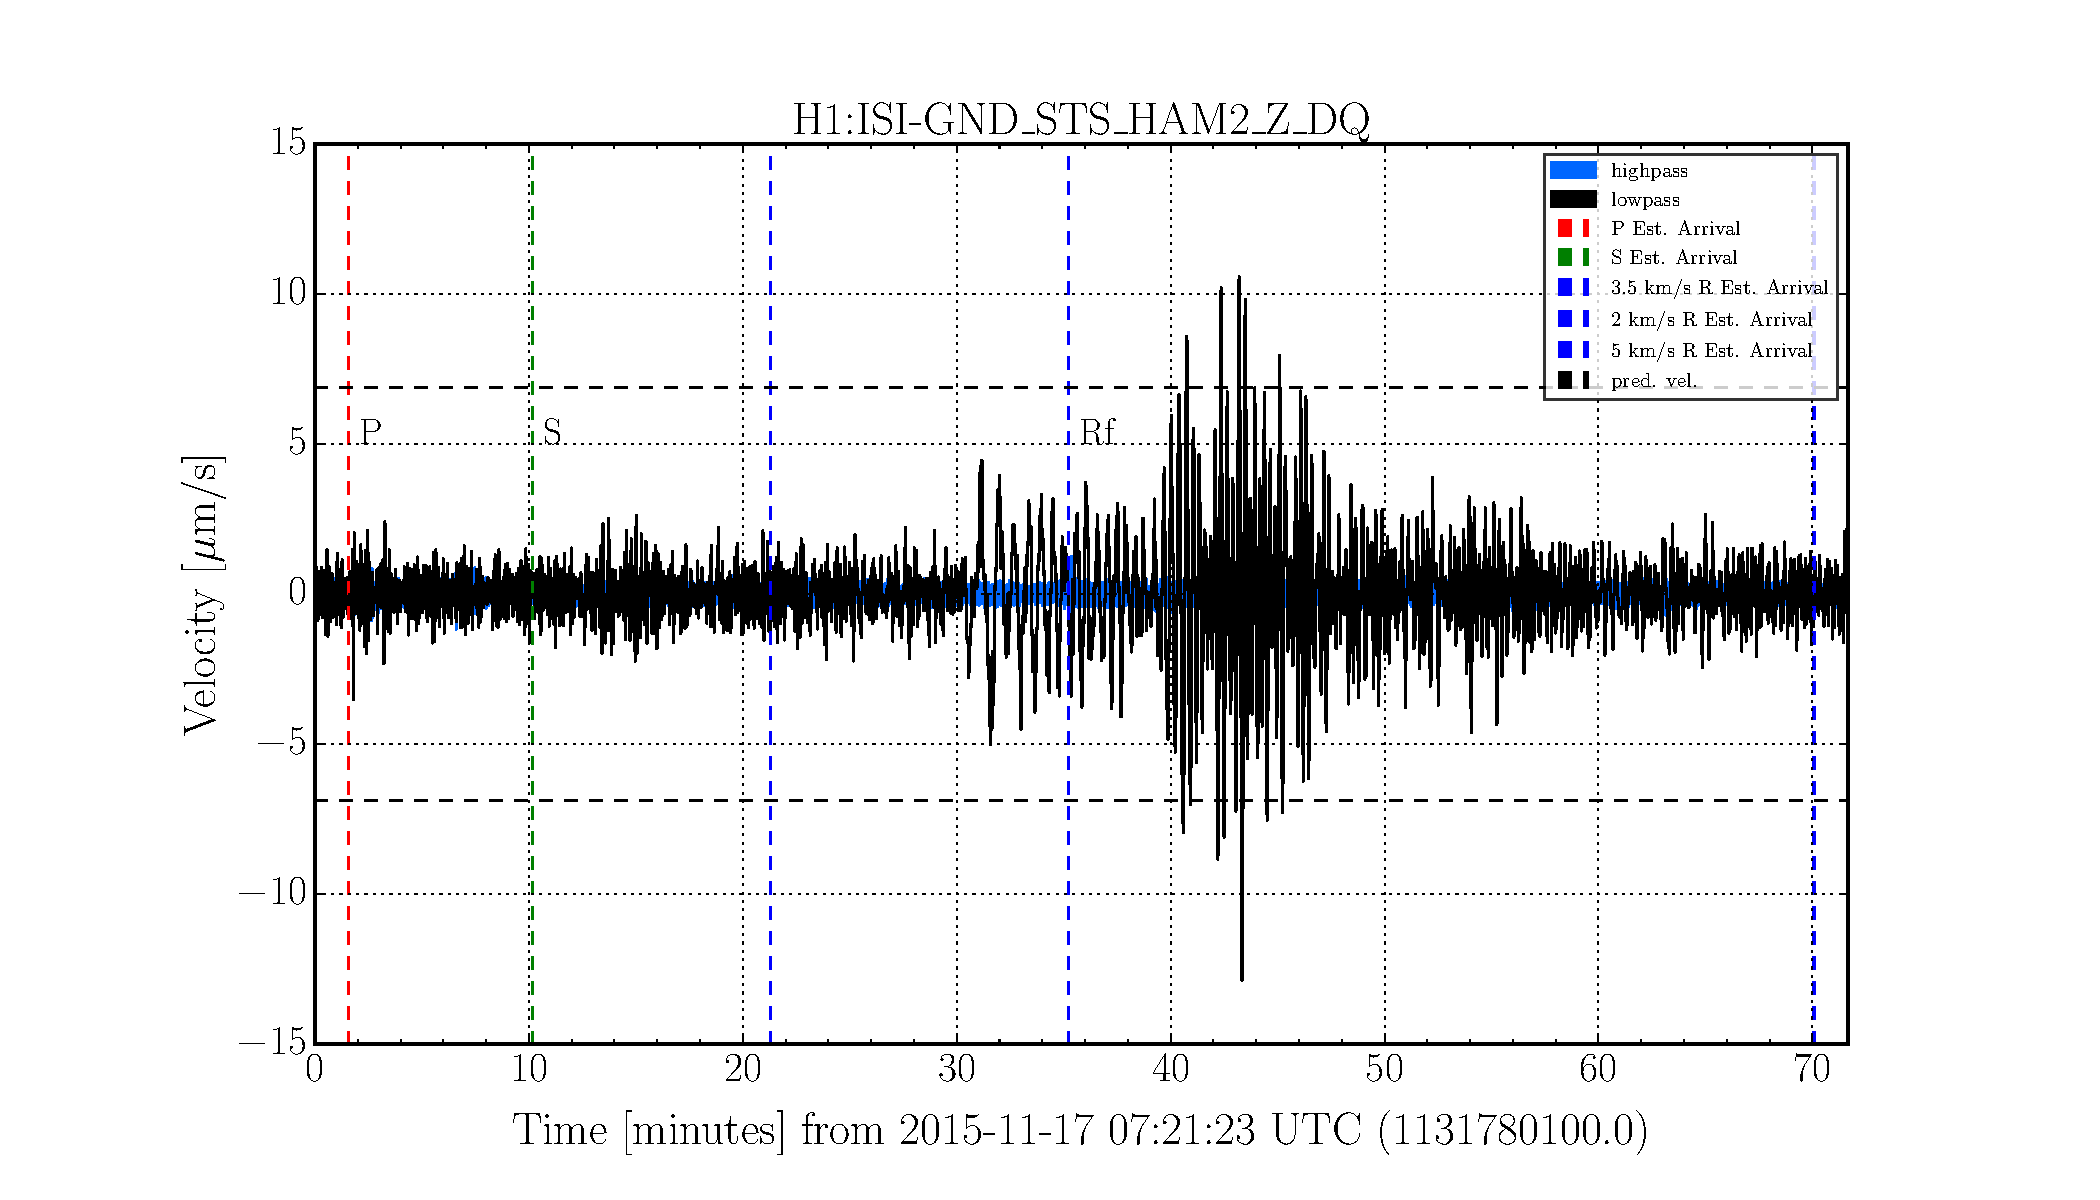
\includegraphics[width=0.99\linewidth]{plots/timeseries.pdf}
Ground motion from a seismometer at the LIGO Hanford site located in Washington, USA for the Nov 17, 2015 6.5 magnitude earthquake in Greece.\\

\begin{itemize}
\item Warning system relies on the most preliminary notices of earthquakes currently available generated by worldwide networks of seismometers. 
\item USGS provides preliminary estimates of the location providing latitude, longitude, and depth of each event.
\item These solutions are distributed through USGS's Product Distribution Layer (PDL), which has been configured to receive notifications for all located earthquakes worldwide. 
\end{itemize}

}

\headerbox{Site Notification}{name=epics,column=0,below=notices}{
\begin{itemize}
\item We use the ground velocity at the site and time-of-arrival predictions to create warnings for the detectors.
\item The algorithm analyzes the recent notifications and places a threshold on the predictions.
\item 
We provide a set of variables that contains the following information: amplitude prediction, probability of lockloss, earthquake time-of-arrival.
\end{itemize}
}

\headerbox{Acknowledgements}{name=acknowledgements,column=0,below=epics, above=bottom}{
\smaller						% Make the whole text smaller
\vspace{-0.4em}			% Save some space at the beginning
MC was supported by the National Science Foundation Graduate Research Fellowship
Program, under NSF grant number DGE 1144152. 
} 

\headerbox{Ground Velocity Prediction}{name=amplitude,span=1,column=1,row=0}{

 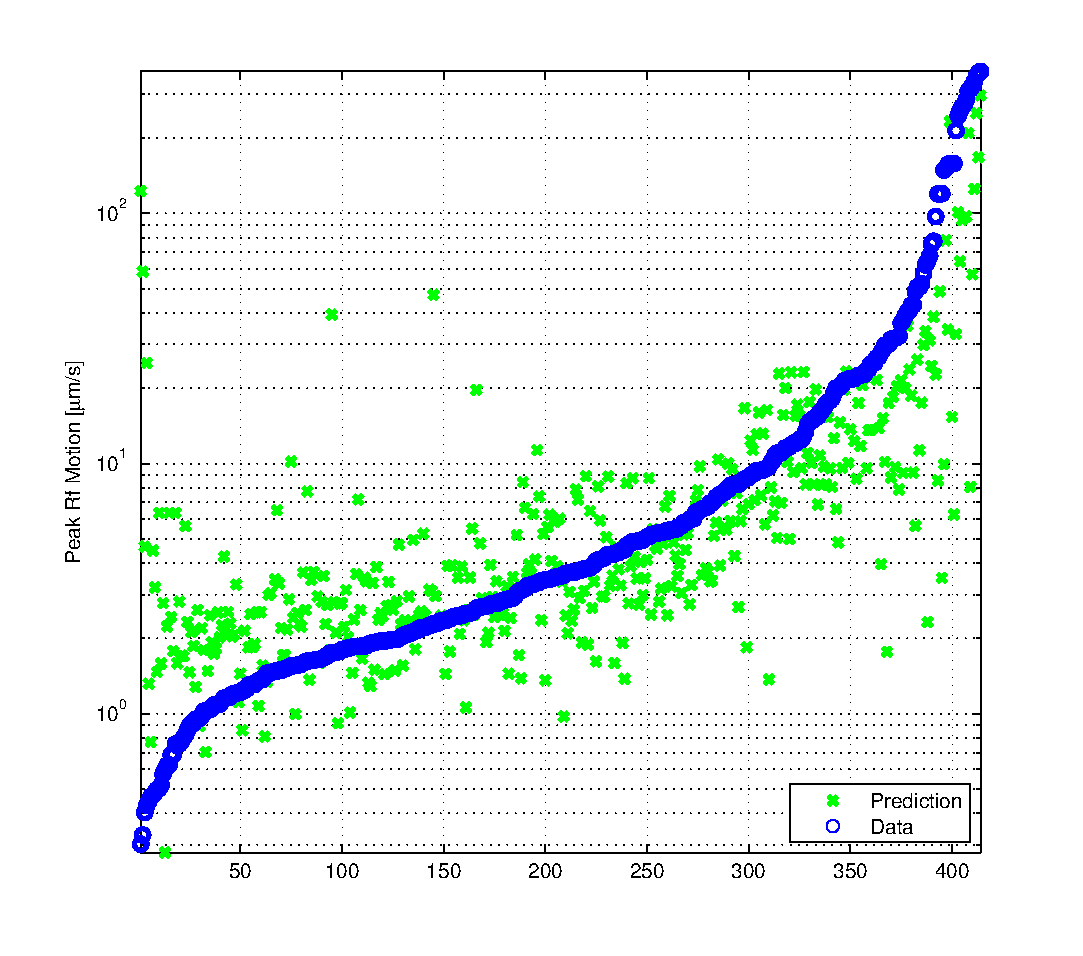
\includegraphics[width=0.99\linewidth]{plots/Prediction_LHO_S5_S6.pdf} \\
Fit of peak velocities seen during S5-S6 at the LIGO Hanford interferometer to equation \ref{eq:Rfamp}.\\

We estimate the peak amplitude of the surface waves, Rf$_{\rm amp}$, at the sites using
\begin{equation}
{\rm Rf_{amp}} = A e^{-2 \pi h f_{\rm c}/c_1}e^{-2 \pi d f_{\rm c}/c_2/Q}/r^{s_1}
\label{eq:Rfamp}
\end{equation}
where $f_{\rm c} = 10^{2.3-M/2}$ is the corner frequency, $A = M A_0/f_c^{s_2}$, $Q=Q_0/f_{\rm c}^{s_3}$, M is the magnitude of the earthquake, d is the distance, h is the depth of the earthquake. The free model parameters are $A_0,\,Q_0,\,c_i,\,s_i$ whose values are derived from minimizing the difference between the amplitude seen at the interferometer and that predicted by the equation.

 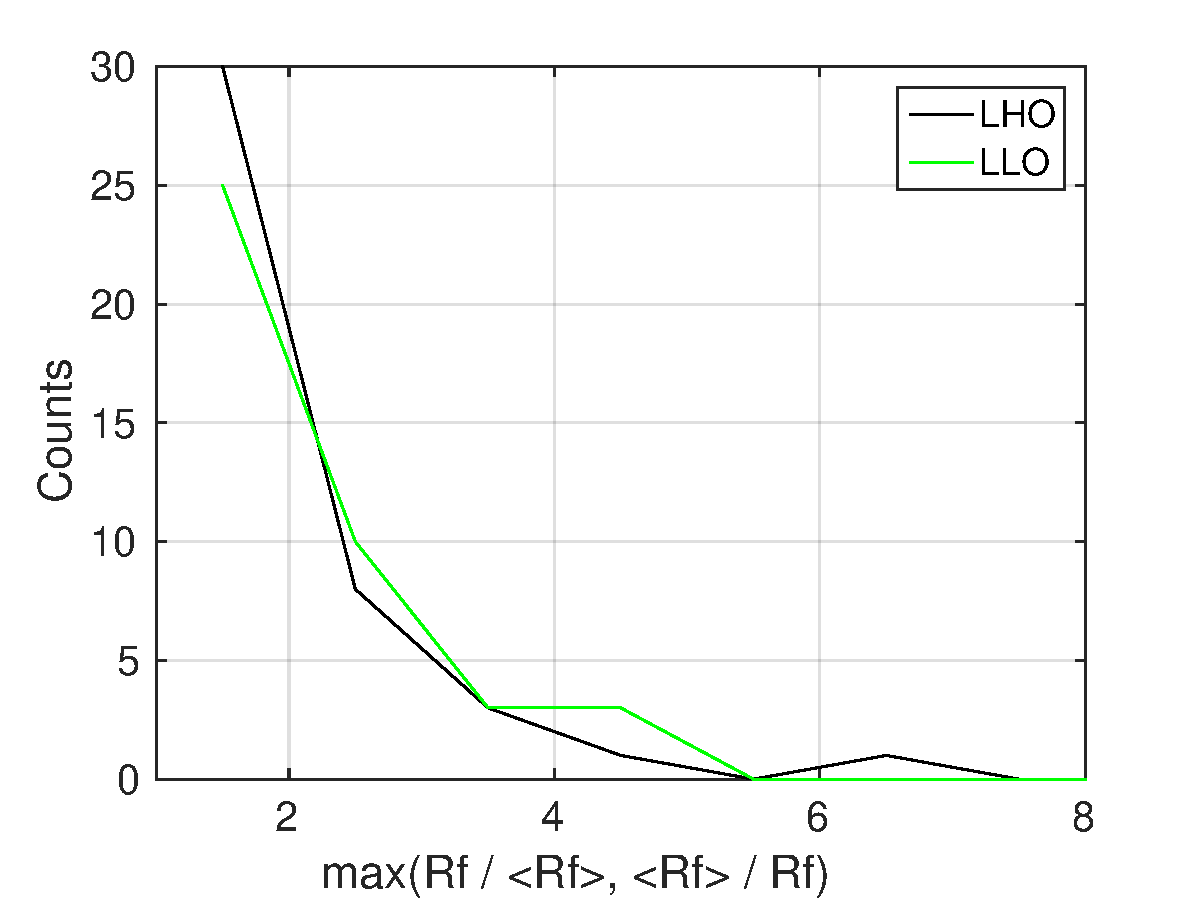
\includegraphics[width=0.99\linewidth]{plots/pred_diff.pdf}
An important quality for an earthquake monitor is the accuracy of the ground-motion amplitude prediction and the time-of-arrival. We show the performance of prediction of peak ground motion seen at the interferometers (LHO and LLO) using fit parameters estimated from previous data. About 94\% of events are within a factor of 5, while those that are not are almost exclusively events that are due to the overlap of multiple events. 

}

\headerbox{Notification latency}
{name=notification,span=1,column=1,below=amplitude,above=bottom}{

 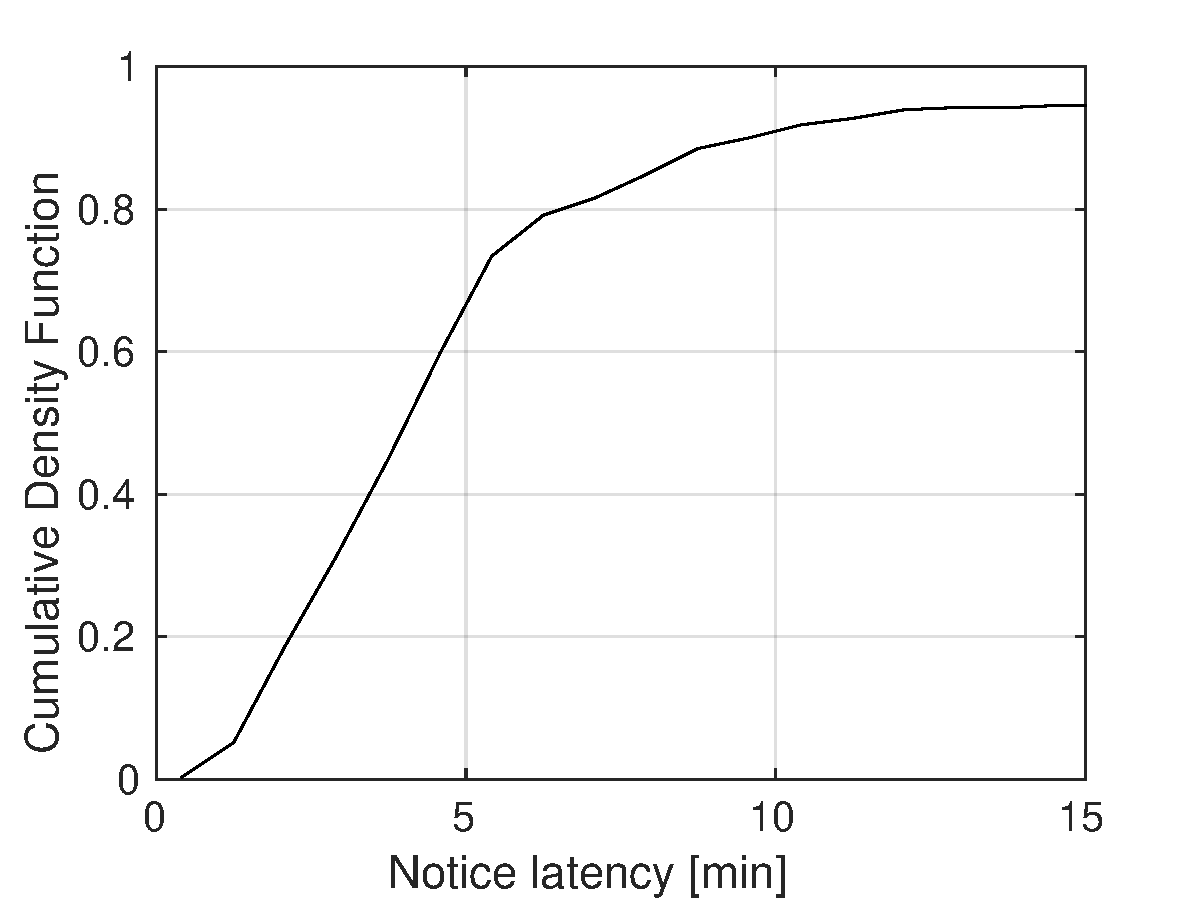
\includegraphics[width=0.49\linewidth]{plots/earthquake_notice.pdf}
 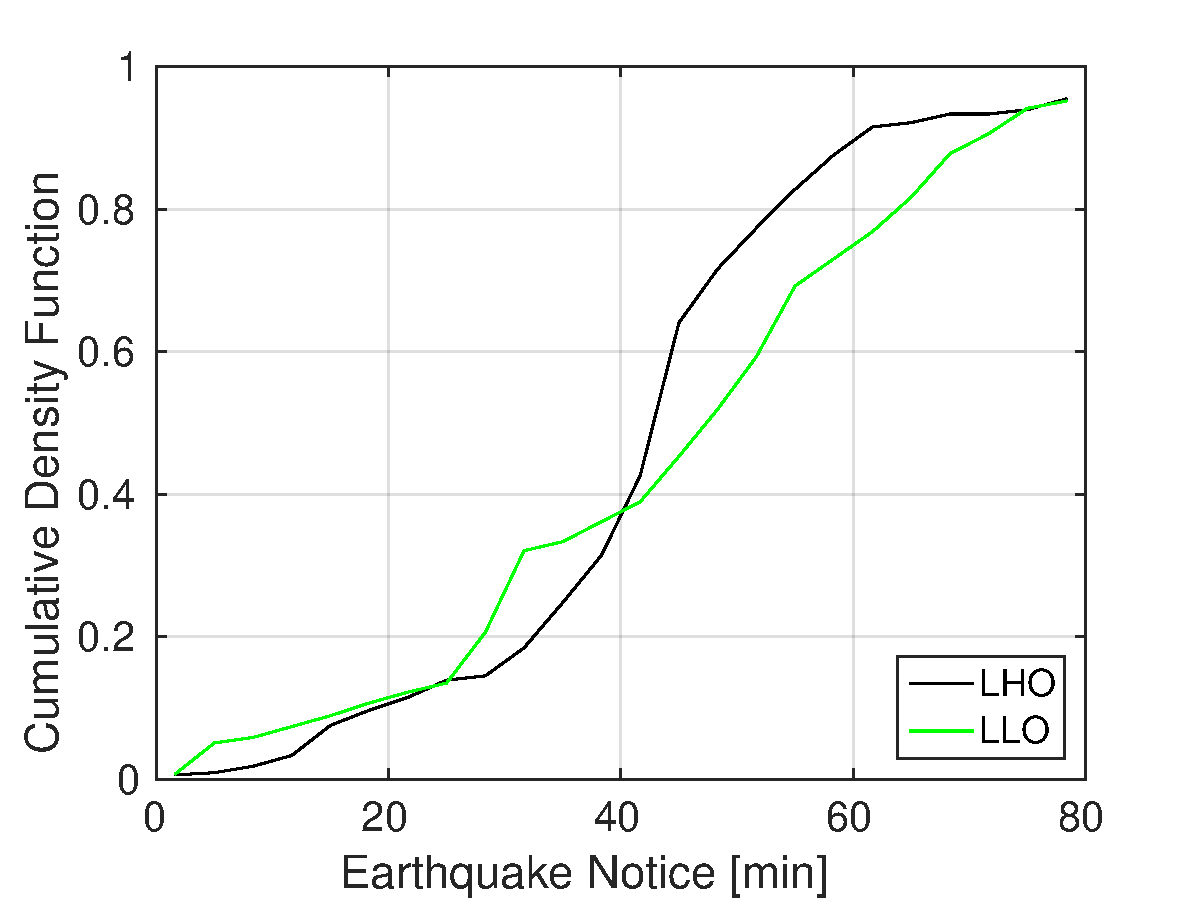
\includegraphics[width=0.49\linewidth]{plots/lockloss_notice.pdf}
 On the left is the time delay between the earthquake and PDL client notification. On the right,
the cumulative probability distribution of time delays between the earthquake and approximate arrival of surface waves, assuming surface wave velocities of 3.5\,km/s. \\


%One of the most important qualities of an earthquake monitor is the notification latency, or the amount of warning time a detector has to respond to incoming seismic waves.
%This is more than sufficient time for gravitational-wave detectors to respond by changing control configurations.

}

\headerbox{Effect of early notices}{name=early,span=1,column=2,row=0}{

 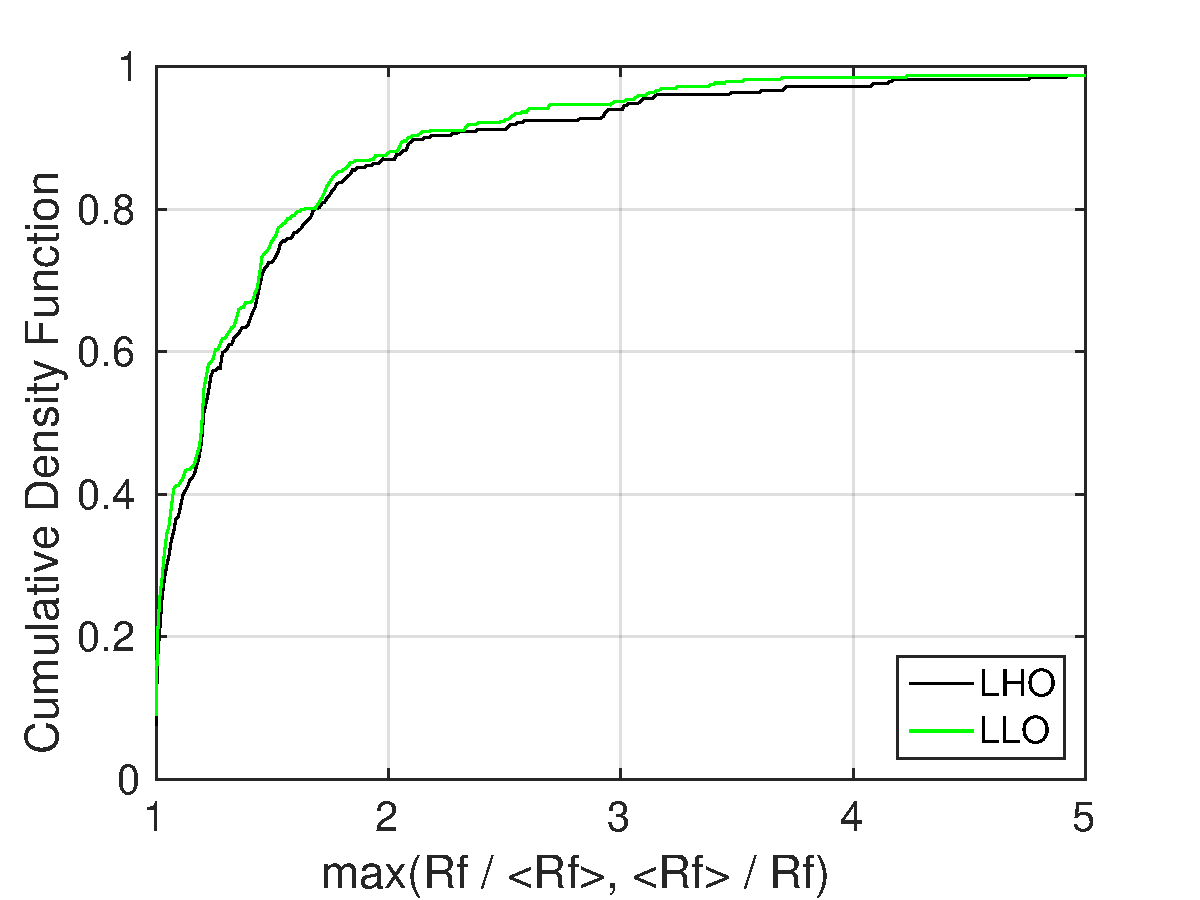
\includegraphics[width=0.49\linewidth]{plots/initial_vs_final.pdf}
 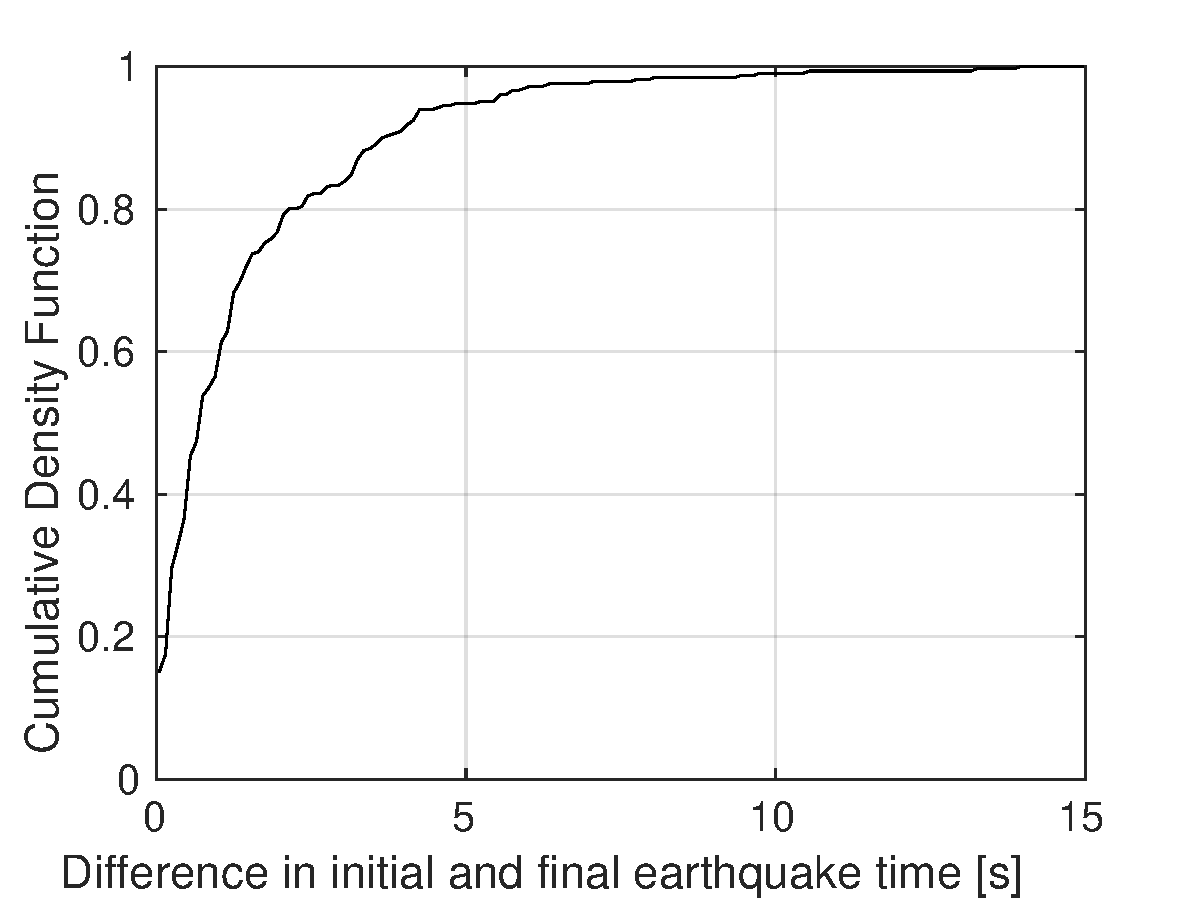
\includegraphics[width=0.49\linewidth]{plots/lockloss_est_timediff.pdf}

We use the earliest available notices for making time-of-arrival and amplitude predictions.
Because the earliest notices may only rely on a few seismometers, the estimates for both magnitude, depth, location, and time can be off.
On the left is the difference of predicted peak amplitudes seen at the interferometers using the initial and final estimates. About 90\% of events are within a factor of 2 of the final predicted value. On the right is the difference between the initial and final estimates of the earthquake time. About 90\% of early estimates are within 4\,s of the final time.
}

\headerbox{Detector Lockloss}{name=lockloss,span=1,column=2,below=early}{

 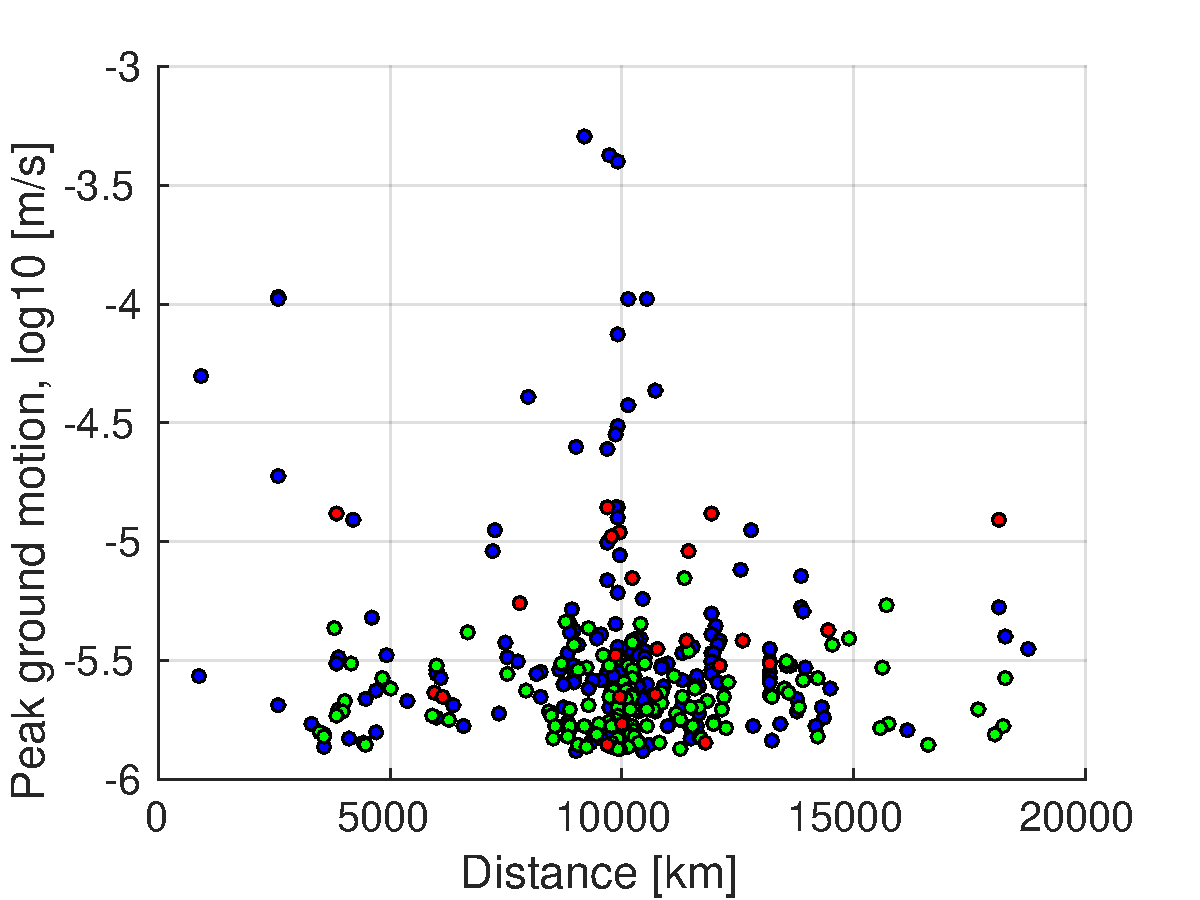
\includegraphics[width=0.49\linewidth]{plots/lockloss_vel_distance_LHO.pdf}
  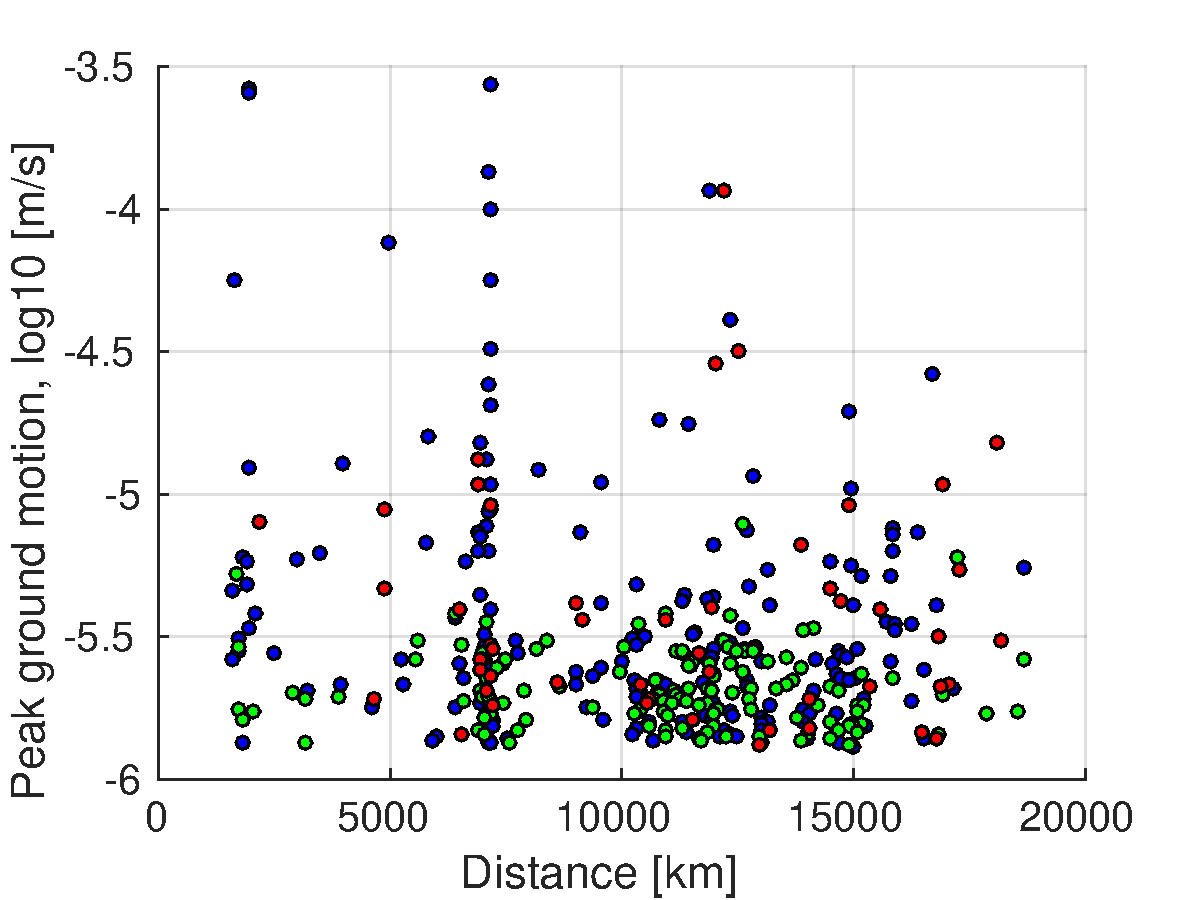
\includegraphics[width=0.49\linewidth]{plots/lockloss_vel_distance_LLO.pdf}
We now measure the amplitude of the seismic ground motion that causes the detector to lose lock.
We show these times, both for those times when lock losses occurred (red), when they did not (green), and when the detector was not locked (blue). 
In general, the plot shows that while in general ground velocities greater than about 5\,$\mu$m/s lead to lock loss, the situation is complicated at lower ground velocities. \\
}

\headerbox{Lockloss prediction performance}{name=ML,span=1,column=2,below=lockloss,above=bottom}{

 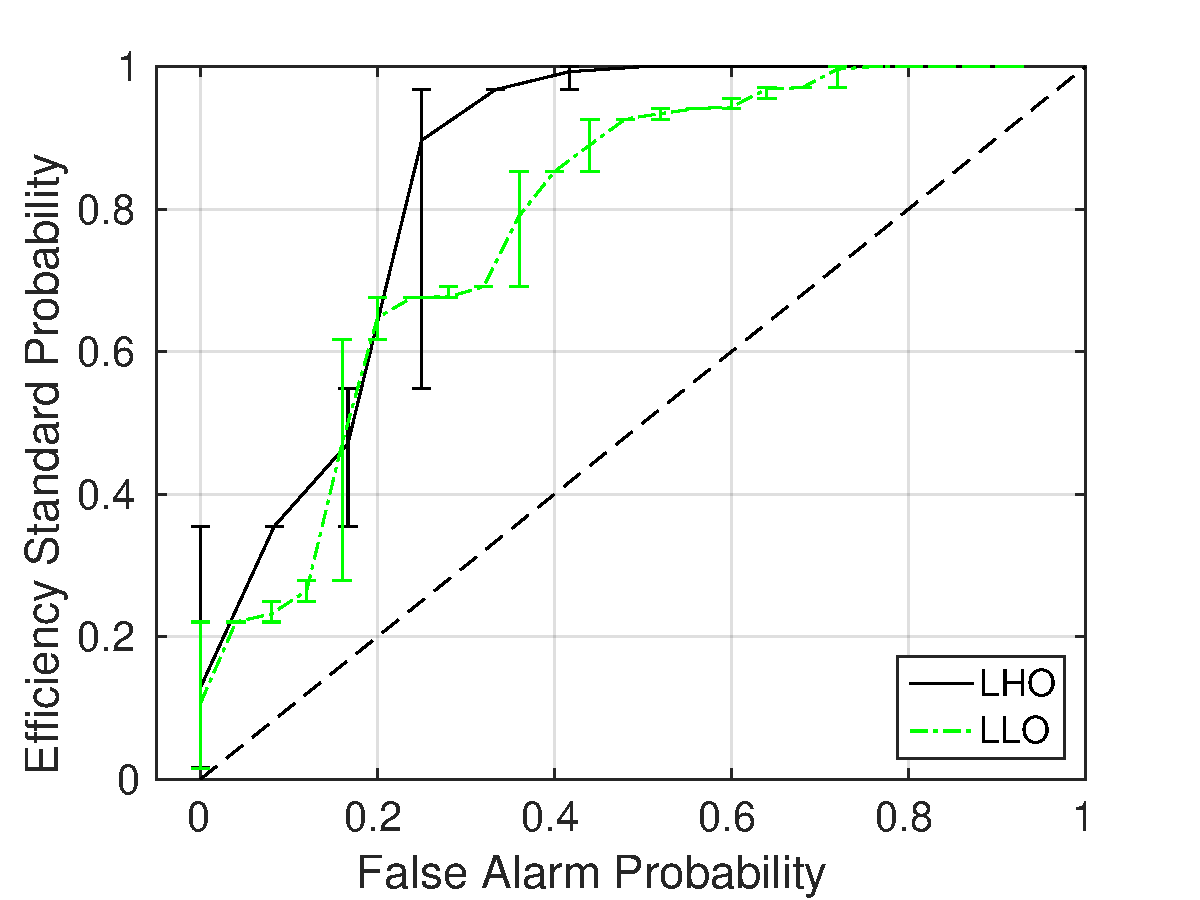
\includegraphics[width=0.99\linewidth]{plots/lockloss_fap_errorbars.pdf}
We use a Machine Learning Algorithm to develop a lockloss prediction model. 
Above, we show the efficiency curves using the earthquake parameters from the PDL client.
The curves which include the observed ground velocity at the sites are similar. 
In general, there is a tradeoff between false alarm probability and efficiency standard probability.
For example, if we adopt a false alarm probability threshold of 0.5, between 90-100\% of earthquakes can be caught.
	
}

\end{poster}
\end{document}
